\documentclass{beamer}
\usepackage[english,russian]{babel}
\usepackage[utf8]{inputenc}
\usepackage{amsmath}
\usepackage{hyperref}
\usetheme{Warsaw}
\usepackage{listings}
\usepackage{xcolor}
\usepackage{tikz}
\usetikzlibrary{graphs}
\usepackage{algorithm}
\usepackage{algpseudocode}

\lstset{
    frame=tb,
    tabsize=4,
    showstringspaces=false,
    numbers=left,
    commentstyle=\color{green},
    keywordstyle=\color{blue},
    stringstyle=\color{red},
    emph={baz},
    emphstyle=\textbf
}

\begin{document}

\title{Задачи разрешимости логических формул и приложения\newline Лекция 5. Алгоритм Conflict-Driven Clause Learning}
\author{Роман Холин}
\institute{Московский государственный университет}
\date{Москва, 2021}

\begin{frame}
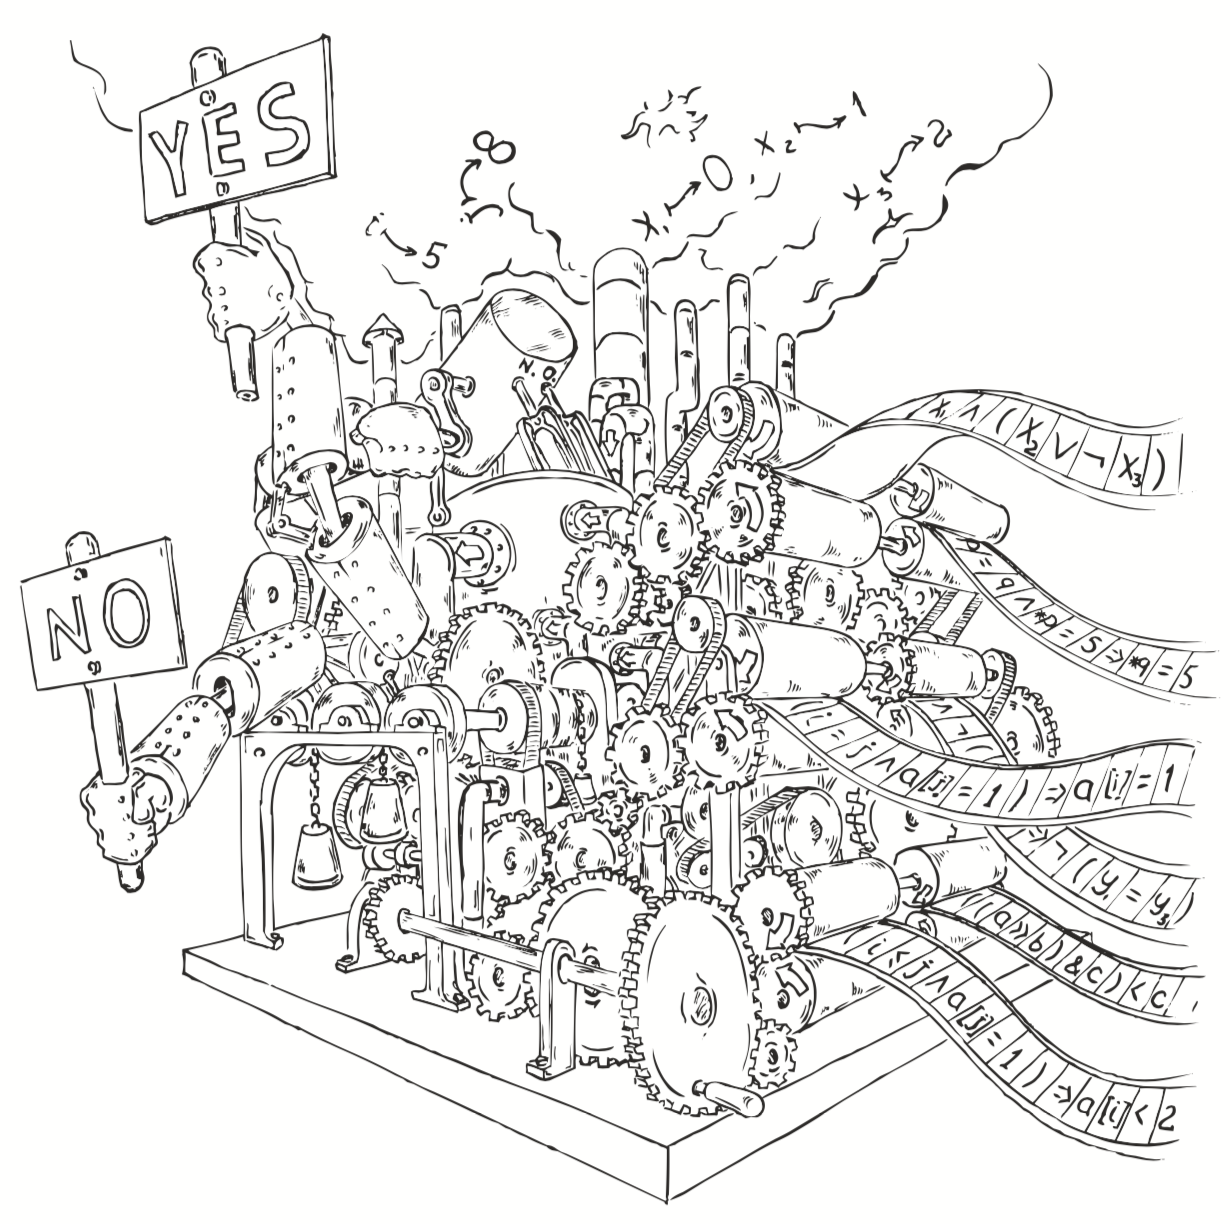
\includegraphics[scale=0.5]{../decision-procedure.png}
\end{frame}

\frame{\titlepage}

\begin{frame}{Элементарный алгоритм}
\begin{itemize}
\item Брутфорс
\item $O(2^n)$
\end{itemize}
\end{frame}

\begin{frame}{Определения}
Пусть произведена частичная оценка.\newline
Дизъюнкт:
\begin{itemize}
\item Выполнимый - если хотя бы один литерал истинен при это частичной оценке
\item Противоречивый - если все литералы дизъюнкта оценены ложны
\item Единичный - если все литералы дизъюнкта, кроме одного, оценены и ложны
\item Неразрешенный - иначе
\end{itemize}
\end{frame}

\begin{frame}{Правило единичного дизъюнкта}
\begin{itemize}
\item В единичном дизъюнкте не оцененный литерал должен быть истиным
\item Единичный дизъюнкт называют предпосылкой для переменной $v$, если она была оценена после применения правила единичного
дизъюнкта для него
\end{itemize}
\end{frame}

\begin{frame}{Conflict-driven clause learning}
\begin{algorithmic}
\Function {CDCL}{}
    \While {true}
        \While {BCP() = "conflict"}
            \State backtrack-level := Analyze-Conflict()
            \If {backtrack-level < 0}
                \State return "Unsatisfiable"
            \EndIf
            \State BackTrack(backtrack-level)
            \If {$\lnot$ Decide()}
                \State return "Satisfiable"
            \EndIf
        \EndWhile
    \EndWhile
\EndFunction
\end{algorithmic}
\end{frame}

\begin{frame}{Описание функций}
\begin{itemize}
\item Decide() - ложь, тогда и только тогда, когда все переменные оценены. Оценивает переменную
\item BCP() - "conflict", тогда и только тогда, когда есть конфликтный дизъюнкт
\item Analyze-Conflict() - на какой уровень принятия решений нужно вернуться. Если "conflict", то добавляет блокирующий
дизъюнкт
\item BackTrack(dl) - устанавливает уровень принятия решений dl и убирает из оценки переменные, которые были вычислены после dl
\end{itemize}
\end{frame}

\begin{frame}{Граф следствий}
\begin{itemize}
\item Будем писать $x_i@dl$, если на уровне принятия решений dl мы присвоили переменной $x_i$ значение истина и $\lnot x_i@dl$ -
если присволи ложь
\item Вершины графа - переменные, определенные частичной оценкой
\item Из $v_i$ идет ребро $v_j$, если $v_j$ оценена в результате BCP() и $v_i$ входит в дизъюнкт-предпосылку $c$. Эти ребра
помечаются меткой $c$
\item Если есть "конфликт", то ему соответствует вершина. Пусть $c$ - конфликтный дизъюнкт. Тогда к вершине "конфликт" идут
ребра от переменных, входящих в $c$ и они помечаются меткой $c$
\end{itemize}
\end{frame}

\begin{frame}
$c_1 = (\lnot x_1 \vee x_2 )$\newline
$c_2 = (\lnot x_1 \vee x_3 \vee x_5 )$\newline
$c_3 = (\lnot x_2 \vee x_4 )$\newline
$c_4 = (\lnot x_3 \vee \lnot x_4 )$\newline
$c_5 = (x_1 \vee x_5 \vee \lnot x_2 )$\newline
$c_6 = (x_2 \vee x_3 )$\newline
$c_7 = (x_2 \vee \lnot x_3 )$\newline
$c_8 = (x_6 \vee \lnot x_5 )$\newline
\end{frame}

\begin{frame}
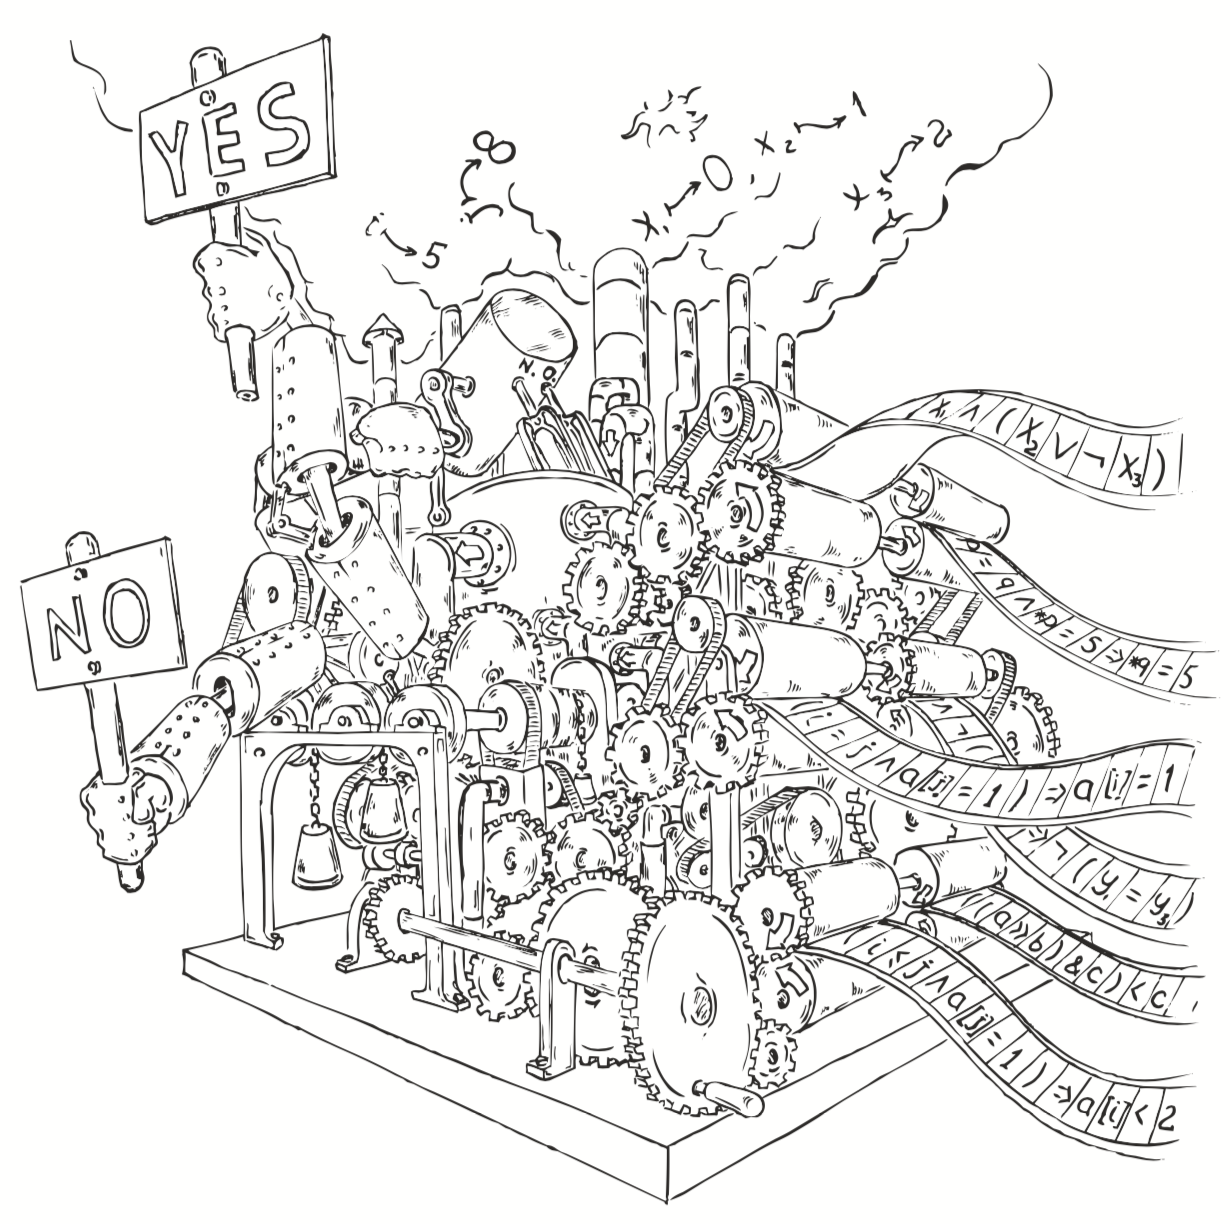
\includegraphics[scale=0.5]{../decision-procedure.png}
\end{frame}

\end{document}
